\chapter{Accelerator SRF Theory and Application}\label{appendix:SRF} 
    
Current state of the art Nb$_3$Sn thin films on Cu are nearing commercialization. Recent progress has shown beyond FCC requirements for accelerator and water treatment applications using Nb$_3$Sn cavities with cyro coolers due to its lower cooling requirements compared to that of bulk Nb. 


    \section{SRF Cavity History (1977-Present)}

    While the superconducting magnet community was gaining momentum, a parallel effort to produce superconducting resonators started in 1961 at the Rutherford High Energy Laboratory in England \cite{banfordFeasibilitySuperconductingProton1961}. The first resonators were made with lead and niobium, but lead is toxic and was abandoned. Nb$_3$Sn cavities also were made early in 1977 by exposing an already prepared Nb cavity with a tin vapor at 1100 $^\circ$C. This cavity's quality factor $Q = 2.7\times10^{9}$ at 4.2 K was a factor of 70$\times$ greater than the best Nb cavity at the time \cite{hillenbrandSuperconductingNbLt1977}. In 1986, a Nb$_3$Sn 500 MHz cavity was made and measured at 4.2 K with a low field $Q$ reaching a value of $2.4\times10^{10}$, and attained an accelerating field of 4.9 MV/m at 5.5 K in the Wuppertal group\cite{arnolds-mayer500MHzSingle1986}. This is a high-quality factor, but because of various material science and engineering challenges associated with Nb$_3$Sn fabrication, the accelerating gradient $E_{\text{acc}}$ of these cavities was limited. The material's surface properties strongly affect the superheating field $H_{\text{sh}}$. 
    
    Although Nb$_3$Sn cavities had promise, they couldn't compete with easy-to-use ductile bulk Nb. Nb cavities became the workhorse for the last 50 years of SRF application and research\cite{Padamsee:2017ohf}. SRF quality factor is determined from a thickness $\sim$3 penetration depths into the cavity, 150nm for Nb and 300nm for Nb$_3$Sn. Therefore, the main scientific thrust in SRF cavity research has been on the surface chemistry of Nb cavities, specifically the oxide formation in the first 10-20 nm. With these modifications to the surface chemistry of Nb, through nitrogen doping\cite{chetriMethodologyCharacterizationSurface2023}, microstructure analysis\cite{Balachandran:2021zuv}, etc. Nb cavities are now nearing the theoretical limit of the material at $Q \sim 10^{11}$ and $E_{acc} = 50$ MeV. Nb as a thin film can be deposited on Cu to increase the quality factor further \cite{Valente-Feliciano:2015qkf}, but $Q$ falls off steeply with higher $E_{\text{acc}}$. More optimization is needed to enhance the microstructure of thin films to possess more bulk-like properties, i.e., fewer impurities and dislocations.
    
    Driven by its potential to surpass the limitations of current Nb on Cu cavities, Nb$_3$Sn is garnering attention once again as a thin-film upgrade, first on an Nb cavity and then on a Cu cavity. Knowledge can be leveraged from Nb thin films on Cu and Nb$_3$Sn superconducting magnets to create an optimized Nb$_3$Sn on Cu.
    
    Nb purification was quickly found out that high purity samples were needed to fully take advantage of the zero resistance state \cite{schirberSuperconductivityEnsuremathAlpha1961}. Niobium was found to have the best properties for a single element \cite{autlerHighFieldSuperconductivityNiobium1962} and was subsequently synthesized with high purity using electron beam melting\cite{Finnemore:1966zz}.
       
    
    %The primary method of cavity-scale Nb$_3$Sn coating has used a vapor diffusion technique where Sn vapor reacts with a bulk Nb cavity at $\sim$1100 °C \cite{Posen:2018zjb}. This route incurs the high cost of making Nb cavities, and the high temperature makes it necessary to apply a thermal conductor such as Cu or Al after the brittle Nb$_3$Sn is formed. Alternative routes starting with copper cavities are possible by evaporating Cu-Sn bronze phases with a reaction at $\sim$700 °C borrowed from the art of manufacturing superconducting Nb$_3$Sn wires\cite{nausInterdiffusionCuSn2000}. 
    
    Nb cavities, the industry standard for high-quality factor cavities, has undergone 50+ years of surface engineering to increase the quality factor from $10^6$ to $10^{10}$. A detailed analysis of the surface chemistry of Niobium oxides and carbides, as well as a comparison of Bulk Nb to that of Surface Nb, was needed to advance to the cavities we have today \cite{chetriMethodologyCharacterizationSurface2023}. We are transitioning into making cavities with both a thin film and more than one element, which requires a comprehensive analysis of thin film microstructure, as well as an understanding of the thermodynamics and kinetics of the compound formation to achieve better results than Nb \cite{Sun:2023ejj}.


        %where the peak electric field amplitude is in the middle of the cavity. Assuming an electron travels at the speed of light, the charged particle enters an accelerating cavity on the axis at $t = 0$ and leaves at time $t = d/c = T_{cav}$. In order for the electron to receive the maximum kick from the resonator, the time it takes the electron to traverse the cavity needs to be one-half an rf period; being,
    
        %\begin{align}
          %  T_{cav} = \frac{d}{c} = \frac{\pi}{\omega_0}.
        %\end{align}
    
       % The amount of average accelerating field 

    %Meissner State SRF (B < Hc1):
       
    %Relevant theories:
    
    %London equations → penetration depth, screening currents
    %Mattis-Bardeen → temperature-dependent surface resistance
    %Geometry optimization → field enhancement, cavity shape
    %
    %NOT relevant:
    
    %Bean critical state
    %Flux flow (Bardeen-Stephen)
    %Flux pinning theories
    %AC flux cutting
    
    %Your Mixed State SRF (B > Hc1):
    %All the flux theories become relevant:
    
    %Bean critical state
    %Bardeen-Stephen flux flow
    %Anderson-Kim creep
    %Coffey-Clem frequency effects
\section{Theory}

    For type I superconductors, the surface energy between normal and superconducting states is positive, and normal regions are not energetically favorable in the bulk of the superconductor. Type II superconductors have a negative surface barrier and, therefore are energetically favorable to admit magnetic flux into the bulk of the superconductor. This comes in the form of quantized magnetic vortices on the length scale of the quantum coherence $\xi$ between the cooper pairs. The cooper pairs lie on the circumference of the vortex and the radius of the vortex is the coherence length $\xi$. Normal electrons are present in the vortex core. This mixed state of normal and superconductor occurs above a critical field $H_{c1}$ and below an upper critical field $H_{c2}$ for a DC field. If a dynamic AC field varies on a time scale smaller than $\approx 10^{-9} s$ \cite{flippenRadialVelocityMagnetic1965} than the time it takes to nucleate a fluxoid $\approx 10^{-6} s$, a vortex will not form. 
    
    This allows for a new critical field, the superheating critical field $H_{sh}$ to exist. A superconductor can exist fully in the Meissner state above $H_{c1}$ up to $H_{sh}$ \cite{matriconSuperheatingFieldsSuperconductors1967}. This frequency-dependent field is termed "super heating" because a nucleation barrier must be overcome to form a fluxoid in the bulk of the material. This is similar to a superheated liquid, where a nucleation site must be present to allow a phase change. When the vortex penetrates the sample fully, the Lorentz force can accelerate the vortex. The core of the vortex has normal electrons, so this movement of normal electrons causes normal ohmic dissipation. These vortices can be pinned by impurities, grain boundaries, etc. and there is a pinning force that must be overcome to depin the vortex. If the pinning force is large, vortex motion is inhibited, and $H_{c2}$ is larger. 


    
    %Check where does this go??
    The superconducting radio frequency (SRF) accelerator community uses cavities at micro-telsa magnetic field while maximizing the RF current. They must keep the surface field below $H_{sh}$ so the cavity doesn't quench. If a vortex is present in high RF current cavities ($high E_{acc}$), as is the case above $H_{sh}$ for particle accelerators, the vortex will feel a huge Lorentz force and causing depinning of the flux lines and depairing of the cooper pairs. This causes flux flow, dissipation, and eventually full breakdown with a quench. Resonating cavities for axion detection in high static magnetic fields are in a very different case. The cavity has no or minimal RF power, with a strong multi-Tesla static magnetic field. This pushes the regime of interest above $H_{sh}$ right below $H_{c2}$. At this field the vortices have almost fully filled the sample, but only feel a small Lorentz force. This small force is not effective at depinning the vertices \cite{campbellResponsePinnedFlux1969}.

Now putting all of this theory together to practically explain RF surface loss when high above $H_{c1}$ with a specific orientation of surface to magnetic field. When a material is in an external magnetic field there is a demagnetization effect which depends on the geometry of the sample. For example with a flat thin sample perpendicular to a magnetic field (Figure.\ref{fig:Demag}(b)), apparent magnetic field felt by the sample is stronger at the edge regions. This results in a demagnetization factor of $D\rightarrow1$ for an infinitely thin film perpendicular to magnet field and $D\rightarrow0$ for the same film parallel to the magnetic field. Therefore the magnetic field felt by the material is:

    \begin{equation}
        \vec{B} = \mu_0 \left(\vec{H} + (1-D) \vec{M}\right) .
        \label{eq:DemagB}
    \end{equation}

    
    \begin{figure}
        \centering
        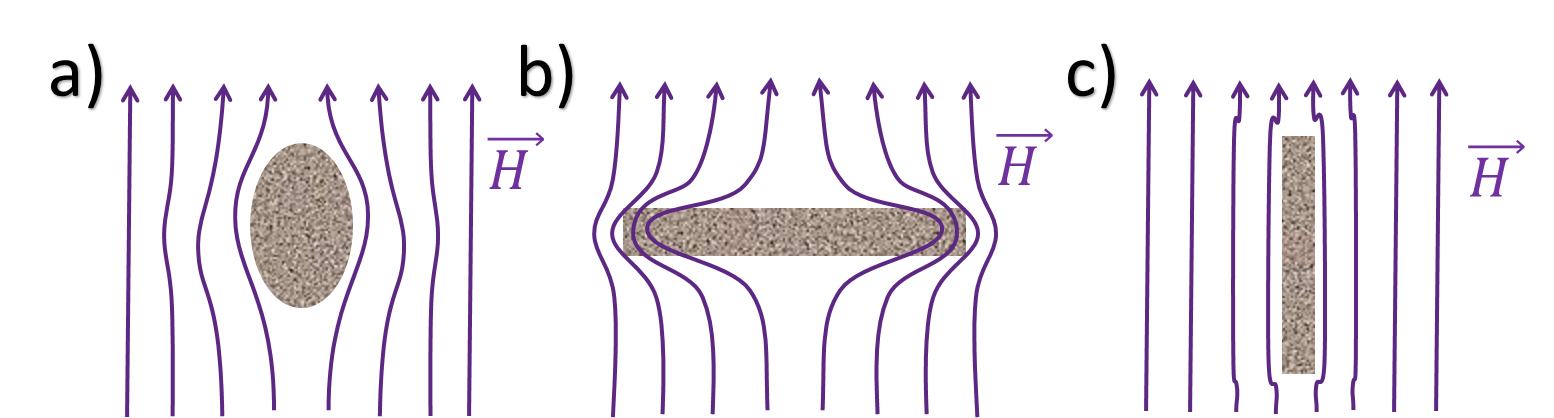
\includegraphics[width=\textwidth]{images/Superconductor/Demag.png}
        \caption{Demagnetization effects in spheroid and flat sample.}{Magnetic field penetration for (a) spheroid and (b) thin film geometries.}
        \label{fig:Demag}
    \end{figure}
     

    For low magnetic field $H<H_{c}$, there is a surface barrier blocking vortex from penetrating the surface, called the Bean-Livingston barrier. At, high magnetic field, 10 T for our application, this barrier is overcome and no longer prevents vortices from entering the sample. However, when demagnetization effects screen the bulk 

     If this electron pair gets further than the coherence length, the electron pair will break. For example, if there is a defect in the material larger than the coherence length, the cooper pair will have trouble sustaining coherent super current across the defect.